\addcontentsline{toc}{subsection}{Differentiability \& Graphing Derivatives}
\subsection*{Differentiability \& Graphing Derivatives}
Recall...
\begin{tcolorbox}[title= DEFINITION OF THE DERIVATIVE OF A FUNCTION,colframe=black,sharp corners,colback=white,colbacktitle=white,coltitle=black,boxrule=1pt]

    The \textbf{derivative} of $f$ at $x$ is given by
    \[f'(x)=\lim_{\Delta x\to0}\frac{f(x+\Delta x)-f(x)}{\Delta x}\]
    provided the limit exists. For all $x$ for which this limit exists, $f'$ is a function of $x$.\\
    \\
    \textbf{Alternate Form:} The derivative of a function $f$ at the point $x=a$ is the limit \[f'(a)=\lim_{x\to a}\frac{f(x)-f(a)}{x-a}\]
    provided the limit exists.
    
\end{tcolorbox}
\vspace{.15cm}
Graphical Representation of the above definitions:

\begin{flushright}
    \begin{tikzpicture}[scale=1]
    
        \draw (-1,0) -- (7.5,0) (0,-.5) -- (0,4.5); % Axis
        \node[below left=2pt and 2pt] at (0,0) {$O$}; % Origin
        
        % Function curve        
        \begin{scope}       
            \clip (-1,0) rectangle (7.5,4.5);
            \draw[line width=1.2pt,smooth,samples=100,domain=-2.5:7.5] plot(\x,{0.3*((\x)-3.5)*((\x)-3.5)+0.5}); 
        \end{scope}
        
        \def\xA{2.5} \def\yA{0.8}
        \coordinate (A) at (\xA,\yA);
        \draw[dashed] (\xA,0) node[below=2pt] {\small $a$} -- (A) -- (0,\yA) node[left] {\small $f(a)$};
                
        \def\xM{6.5} \def\yM{3.2}
        \coordinate (M) at (\xM,\yM);
        \draw[dashed] (\xM,0) node[below] {\small $a+\Delta x$} -- (M) -- (0,\yM) node[left] {\small $f(a+\Delta x)$};
        \begin{scope}       
            \clip (0.5,-0.5) rectangle (7.5,4.5);

            % Series of lines all through point A
            \foreach \xN/\yN in {6.5/3.2,6/2.38,5.5/1.7,5/1.18,4.5/0.8,4/0.58,3.5/0.5}
                {
                \coordinate (N) at (\xN,\yN);
                \tkzDrawPoint[size=3](N)
                \tkzDrawLine[add=2 and 3,color=gray](A,N)
                }   
        \end{scope}
        
        \draw[line width=1.2pt,color=gray!50!black,smooth,samples=100,domain=0.5:5] plot(\x,{-0.6*(\x)+2.3}) node[above] {$T$};            
        
        \tkzDrawPoints[size=3](A,M)
        \tkzLabelPoint[above=3pt](A)
        \tkzLabelPoint[above left](M)
        
        %%%%Arrows alongside the curve
        \foreach \a/\b in {6.55/6.9, 6/6.35, 5.5/5.85, 4.9/5.35, 4.35/4.75}
            {
            \draw[<-,>=stealth,line width=1pt,color=gray!50!white,smooth,samples=100,domain=\a:\b] plot(\x,{0.32*((\x)-3.95)*((\x)-3.95)+0.55});
            }
        
    \end{tikzpicture}
\end{flushright}

\vspace{\stretch{1}}

Consider the function $y=\begin{cases}
                        x^2 & x\le0\\ 2x & x>0
                        \end{cases}$. What is the derivative of the function at $x=0$?
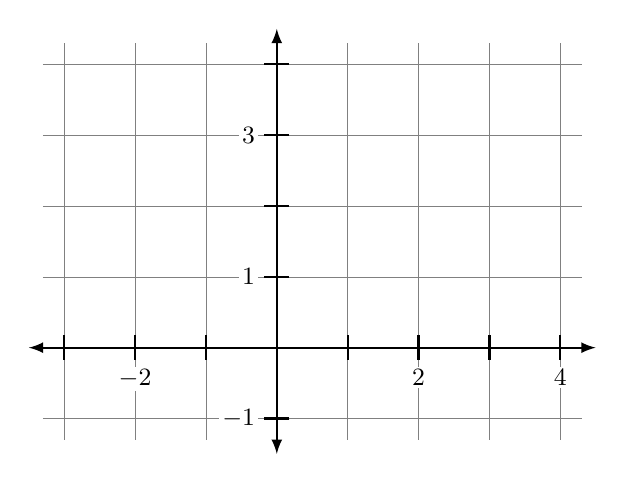
\begin{tikzpicture}[xscale=.9,yscale=.9]
    \draw[step=1,style=help lines,] (-3.3,-1.3) grid (4.3,4.3);
    \draw[latex-latex, thick] (-3.5,0)--(4.5,0);
    \draw[latex-latex, thick] (0,-1.5)--(0,4.5);
    \foreach \x in {-2,2,4}
        \draw[thick] (\x,5pt) -- (\x,-5pt) node [below=.7mm,fill=white,inner sep=1pt] {\small$\x$};
    \foreach \y in {-1,1,3}
        \draw[thick] (5pt,\y) -- (-5pt,\y) node [left=.7mm,fill=white,inner sep=1pt] {\small$\y$};
    \foreach \x in {-3,-1,1,3}
        \draw[thick] (\x,5pt) -- (\x,-5pt);
    \foreach \y in {2,4}
        \draw[thick] (5pt,\y) -- (-5pt,\y);
\end{tikzpicture}


\newpage

\noindent\textbf{Four Instances where a Derivative will Fail to Exist:}
\begin{questions}
    
    \begin{minipage}[t]{0.45\linewidth}
        \question At a \textbf{corner}, where the one-sided derivatives differ.\\
        \begin{center}
            Example: $f(x)=|x|$
            
            \vspace{2.5mm}
            
            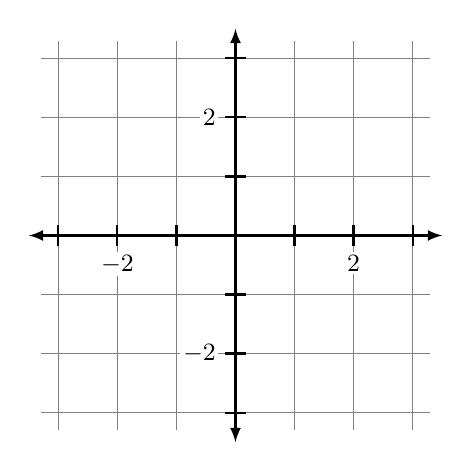
\begin{tikzpicture}[xscale=.75,yscale=.75]
                \draw[step=1,style=help lines,] (-3.3,-3.3) grid (3.3,3.3);
                \draw[latex-latex, thick] (-3.5,0)--(3.5,0);
                \draw[latex-latex, thick] (0,-3.5)--(0,3.5);
                \foreach \x in {-2,2}
                    \draw[thick] (\x,5pt) -- (\x,-5pt) node [below=.7mm,fill=white,inner sep=1pt] {\small$\x$};
                \foreach \y in {-2,2}
                    \draw[thick] (5pt,\y) -- (-5pt,\y) node [left=.7mm,fill=white,inner sep=1pt] {\small$\y$};
                \foreach \x in {-3,-1,1,3}
                    \draw[thick] (\x,5pt) -- (\x,-5pt);
                \foreach \y in {-1,1,-3,3}
                    \draw[thick] (5pt,\y) -- (-5pt,\y);
            \end{tikzpicture}
        \end{center}
    \end{minipage}
    \hfill
    \begin{minipage}[t]{0.45\linewidth}
        \question At a \textbf{cusp}, where the slopes of the secant lines approach $\infty$ from one side and $-\infty$ from the other. 
        \begin{center}
            Example: $f(x)=x^{2/3}$
            
            \vspace{2mm}
            
            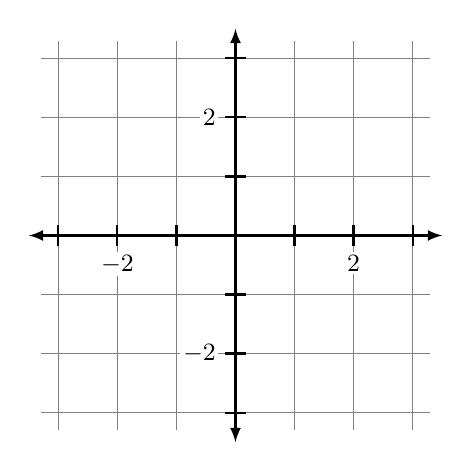
\begin{tikzpicture}[xscale=.75,yscale=.75]
                \draw[step=1,style=help lines,] (-3.3,-3.3) grid (3.3,3.3);
                \draw[latex-latex, thick] (-3.5,0)--(3.5,0);
                \draw[latex-latex, thick] (0,-3.5)--(0,3.5);
                \foreach \x in {-2,2}
                    \draw[thick] (\x,5pt) -- (\x,-5pt) node [below=.7mm,fill=white,inner sep=1pt] {\small$\x$};
                \foreach \y in {-2,2}
                    \draw[thick] (5pt,\y) -- (-5pt,\y) node [left=.7mm,fill=white,inner sep=1pt] {\small$\y$};
                \foreach \x in {-3,-1,1,3}
                    \draw[thick] (\x,5pt) -- (\x,-5pt);
                \foreach \y in {-1,1,-3,3}
                    \draw[thick] (5pt,\y) -- (-5pt,\y);
            \end{tikzpicture}
        \end{center}
    \end{minipage}
    
    
    \begin{minipage}[t]{0.45\linewidth}
        \question At a \textbf{vertical tangent}, where the slopes of the secant lines approach either $\infty$ or $-\infty$ from both sides.
        \begin{center}
            Example: $f(x)=\sqrt[3]{x}$
            
            \vspace{2.5mm}
            
            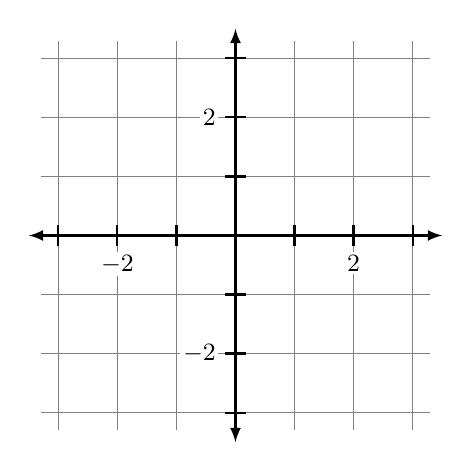
\begin{tikzpicture}[xscale=.75,yscale=.75]
                \draw[step=1,style=help lines,] (-3.3,-3.3) grid (3.3,3.3);
                \draw[latex-latex, thick] (-3.5,0)--(3.5,0);
                \draw[latex-latex, thick] (0,-3.5)--(0,3.5);
                \foreach \x in {-2,2}
                    \draw[thick] (\x,5pt) -- (\x,-5pt) node [below=.7mm,fill=white,inner sep=1pt] {\small$\x$};
                \foreach \y in {-2,2}
                    \draw[thick] (5pt,\y) -- (-5pt,\y) node [left=.7mm,fill=white,inner sep=1pt] {\small$\y$};
                \foreach \x in {-3,-1,1,3}
                    \draw[thick] (\x,5pt) -- (\x,-5pt);
                \foreach \y in {-1,1,-3,3}
                    \draw[thick] (5pt,\y) -- (-5pt,\y);
            \end{tikzpicture}
        \end{center}
    \end{minipage}
    \hfill
    \begin{minipage}[t]{0.45\linewidth}
        \question At a \textbf{point of discontinuity}.
        
        \vspace{3.3mm}
        
        \begin{center}
            Example: $f(x)=\begin{cases}
            -1 & x<0\\ 1 & x\ge0
            \end{cases}$
            
            \vspace{2mm}
            
            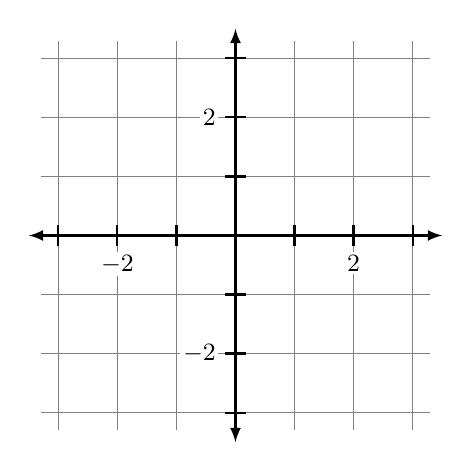
\begin{tikzpicture}[xscale=.75,yscale=.75]
                \draw[step=1,style=help lines,] (-3.3,-3.3) grid (3.3,3.3);
                \draw[latex-latex, thick] (-3.5,0)--(3.5,0);
                \draw[latex-latex, thick] (0,-3.5)--(0,3.5);
                \foreach \x in {-2,2}
                    \draw[thick] (\x,5pt) -- (\x,-5pt) node [below=.7mm,fill=white,inner sep=1pt] {\small$\x$};
                \foreach \y in {-2,2}
                    \draw[thick] (5pt,\y) -- (-5pt,\y) node [left=.7mm,fill=white,inner sep=1pt] {\small$\y$};
                \foreach \x in {-3,-1,1,3}
                    \draw[thick] (\x,5pt) -- (\x,-5pt);
                \foreach \y in {-1,1,-3,3}
                    \draw[thick] (5pt,\y) -- (-5pt,\y);
            \end{tikzpicture}
        \end{center}
    \end{minipage}

\end{questions}

\vfill

\begin{center}
    \begin{itemize}
        \item \textbf{A function must be continuous at \textit{a} to be differentiable at \textit{a}.}
        \item \textbf{If a function is continuous at \textit{a}, that does not mean that it is differentiable.}
        \item \textbf{If a function is differentiable at \textit{a}, then the function is continuous at \textit{a}.}
    \end{itemize}
\end{center}

\vfill

\newpage


The derivative at a point is the slope of the line tangent to the curve at that point. We use this fact to graph derivatives of functions.\\
\\
\noindent\textbf{Examples:}\\
Graph $\displaystyle f(x)=(x-2)^2+1$, then graph the derivative of the function.

\begin{minipage}[t]{0.45\linewidth}
    \begin{center}
        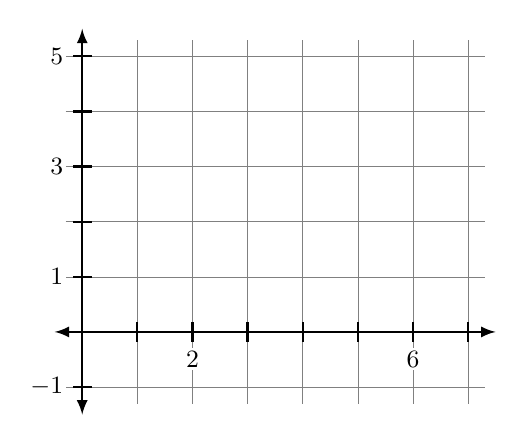
\begin{tikzpicture}[xscale=.7,yscale=.7]
            \draw[step=1,style=help lines,] (-0.3,-1.3) grid (7.3,5.3);
            \draw[latex-latex, thick] (-.5,0)--(7.5,0);
            \draw[latex-latex, thick] (0,-1.5)--(0,5.5);
            \foreach \x in {2,6}
                \draw[thick] (\x,5pt) -- (\x,-5pt) node [below=.7mm,fill=white,inner sep=1pt] {\small$\x$};
            \foreach \y in {-1,1,3,5}
                \draw[thick] (5pt,\y) -- (-5pt,\y) node [left=.7mm,fill=white,inner sep=1pt] {\small$\y$};
            \foreach \x in {1,3,4,5,7}
                \draw[thick] (\x,5pt) -- (\x,-5pt);
            \foreach \y in {2,4}
                \draw[thick] (5pt,\y) -- (-5pt,\y);
        \end{tikzpicture}
    \end{center}
\end{minipage}
\hfill
\begin{minipage}[t]{0.45\linewidth}
    \begin{center}
        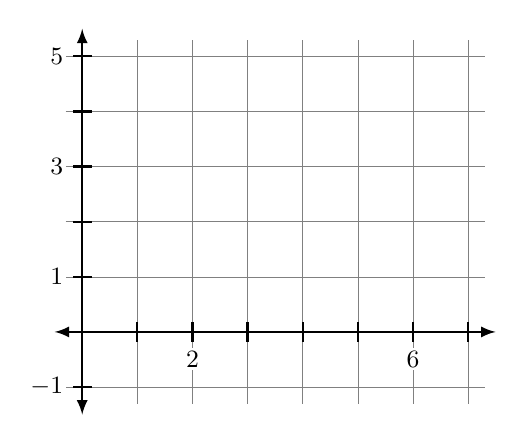
\begin{tikzpicture}[xscale=.7,yscale=.7]
            \draw[step=1,style=help lines,] (-0.3,-1.3) grid (7.3,5.3);
            \draw[latex-latex, thick] (-.5,0)--(7.5,0);
            \draw[latex-latex, thick] (0,-1.5)--(0,5.5);
            \foreach \x in {2,6}
                \draw[thick] (\x,5pt) -- (\x,-5pt) node [below=.7mm,fill=white,inner sep=1pt] {\small$\x$};
            \foreach \y in {-1,1,3,5}
                \draw[thick] (5pt,\y) -- (-5pt,\y) node [left=.7mm,fill=white,inner sep=1pt] {\small$\y$};
            \foreach \x in {1,3,4,5,7}
                \draw[thick] (\x,5pt) -- (\x,-5pt);
            \foreach \y in {2,4}
                \draw[thick] (5pt,\y) -- (-5pt,\y);
        \end{tikzpicture}
    \end{center}
\end{minipage}


Graph a positive cubic function passing through the point $(0,\,1)$ and having a maximum at $(2,\,4)$ and a minimum at $(6,\,1)$. Graph the derivative of the function.

\begin{minipage}[t]{0.45\linewidth}
    \begin{center}
        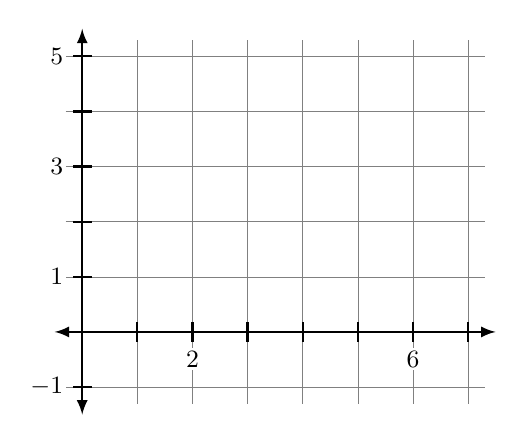
\begin{tikzpicture}[xscale=.7,yscale=.7]
            \draw[step=1,style=help lines,] (-0.3,-1.3) grid (7.3,5.3);
            \draw[latex-latex, thick] (-.5,0)--(7.5,0);
            \draw[latex-latex, thick] (0,-1.5)--(0,5.5);
            \foreach \x in {2,6}
                \draw[thick] (\x,5pt) -- (\x,-5pt) node [below=.7mm,fill=white,inner sep=1pt] {\small$\x$};
            \foreach \y in {-1,1,3,5}
                \draw[thick] (5pt,\y) -- (-5pt,\y) node [left=.7mm,fill=white,inner sep=1pt] {\small$\y$};
            \foreach \x in {1,3,4,5,7}
                \draw[thick] (\x,5pt) -- (\x,-5pt);
            \foreach \y in {2,4}
                \draw[thick] (5pt,\y) -- (-5pt,\y);
        \end{tikzpicture}
    \end{center}
\end{minipage}
\hfill
\begin{minipage}[t]{0.45\linewidth}
    \begin{center}
        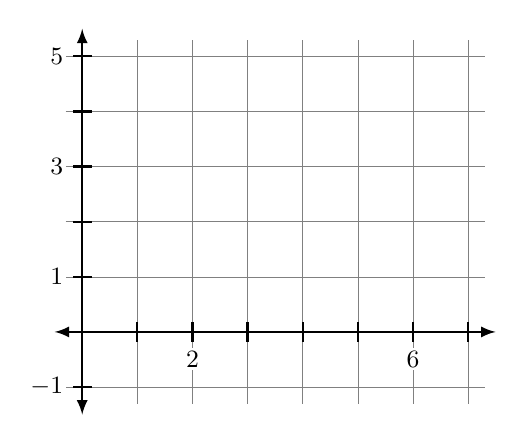
\begin{tikzpicture}[xscale=.7,yscale=.7]
            \draw[step=1,style=help lines,] (-0.3,-1.3) grid (7.3,5.3);
            \draw[latex-latex, thick] (-.5,0)--(7.5,0);
            \draw[latex-latex, thick] (0,-1.5)--(0,5.5);
            \foreach \x in {2,6}
                \draw[thick] (\x,5pt) -- (\x,-5pt) node [below=.7mm,fill=white,inner sep=1pt] {\small$\x$};
            \foreach \y in {-1,1,3,5}
                \draw[thick] (5pt,\y) -- (-5pt,\y) node [left=.7mm,fill=white,inner sep=1pt] {\small$\y$};
            \foreach \x in {1,3,4,5,7}
                \draw[thick] (\x,5pt) -- (\x,-5pt);
            \foreach \y in {2,4}
                \draw[thick] (5pt,\y) -- (-5pt,\y);
        \end{tikzpicture}
    \end{center}
\end{minipage}


Now let's try it backwards!!!  Graph $\displaystyle f'(x)=\begin{cases}
2 & x>1\\ -1 & x<1
\end{cases}$ below. Given that $f(0)=0$ and $f(x)$ is continuous, graph $f(x)$.

\begin{minipage}[t]{0.45\linewidth}
    \begin{center}
        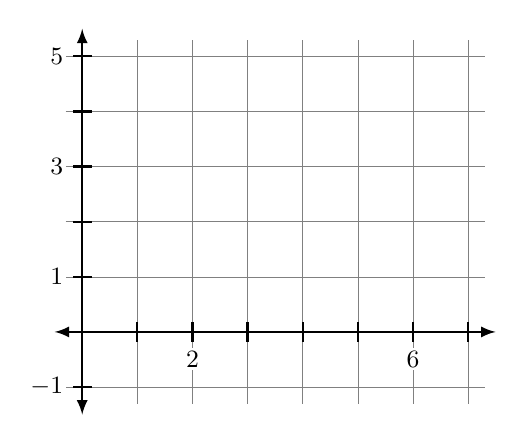
\begin{tikzpicture}[xscale=.7,yscale=.7]
            \draw[step=1,style=help lines,] (-0.3,-1.3) grid (7.3,5.3);
            \draw[latex-latex, thick] (-.5,0)--(7.5,0);
            \draw[latex-latex, thick] (0,-1.5)--(0,5.5);
            \foreach \x in {2,6}
                \draw[thick] (\x,5pt) -- (\x,-5pt) node [below=.7mm,fill=white,inner sep=1pt] {\small$\x$};
            \foreach \y in {-1,1,3,5}
                \draw[thick] (5pt,\y) -- (-5pt,\y) node [left=.7mm,fill=white,inner sep=1pt] {\small$\y$};
            \foreach \x in {1,3,4,5,7}
                \draw[thick] (\x,5pt) -- (\x,-5pt);
            \foreach \y in {2,4}
                \draw[thick] (5pt,\y) -- (-5pt,\y);
        \end{tikzpicture}
    \end{center}
\end{minipage}
\hfill
\begin{minipage}[t]{0.45\linewidth}
    \begin{center}
        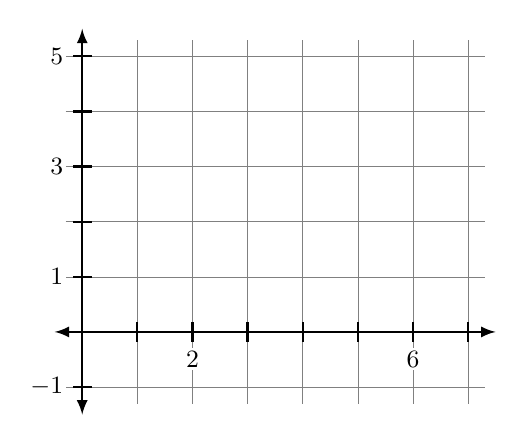
\begin{tikzpicture}[xscale=.7,yscale=.7]
            \draw[step=1,style=help lines,] (-0.3,-1.3) grid (7.3,5.3);
            \draw[latex-latex, thick] (-.5,0)--(7.5,0);
            \draw[latex-latex, thick] (0,-1.5)--(0,5.5);
            \foreach \x in {2,6}
                \draw[thick] (\x,5pt) -- (\x,-5pt) node [below=.7mm,fill=white,inner sep=1pt] {\small$\x$};
            \foreach \y in {-1,1,3,5}
                \draw[thick] (5pt,\y) -- (-5pt,\y) node [left=.7mm,fill=white,inner sep=1pt] {\small$\y$};
            \foreach \x in {1,3,4,5,7}
                \draw[thick] (\x,5pt) -- (\x,-5pt);
            \foreach \y in {2,4}
                \draw[thick] (5pt,\y) -- (-5pt,\y);
        \end{tikzpicture}
    \end{center}
\end{minipage}



\newpage
